\part{Design}
\label{part:design}

\begin{frame}
\vspace{-1em}
\begin{center}
	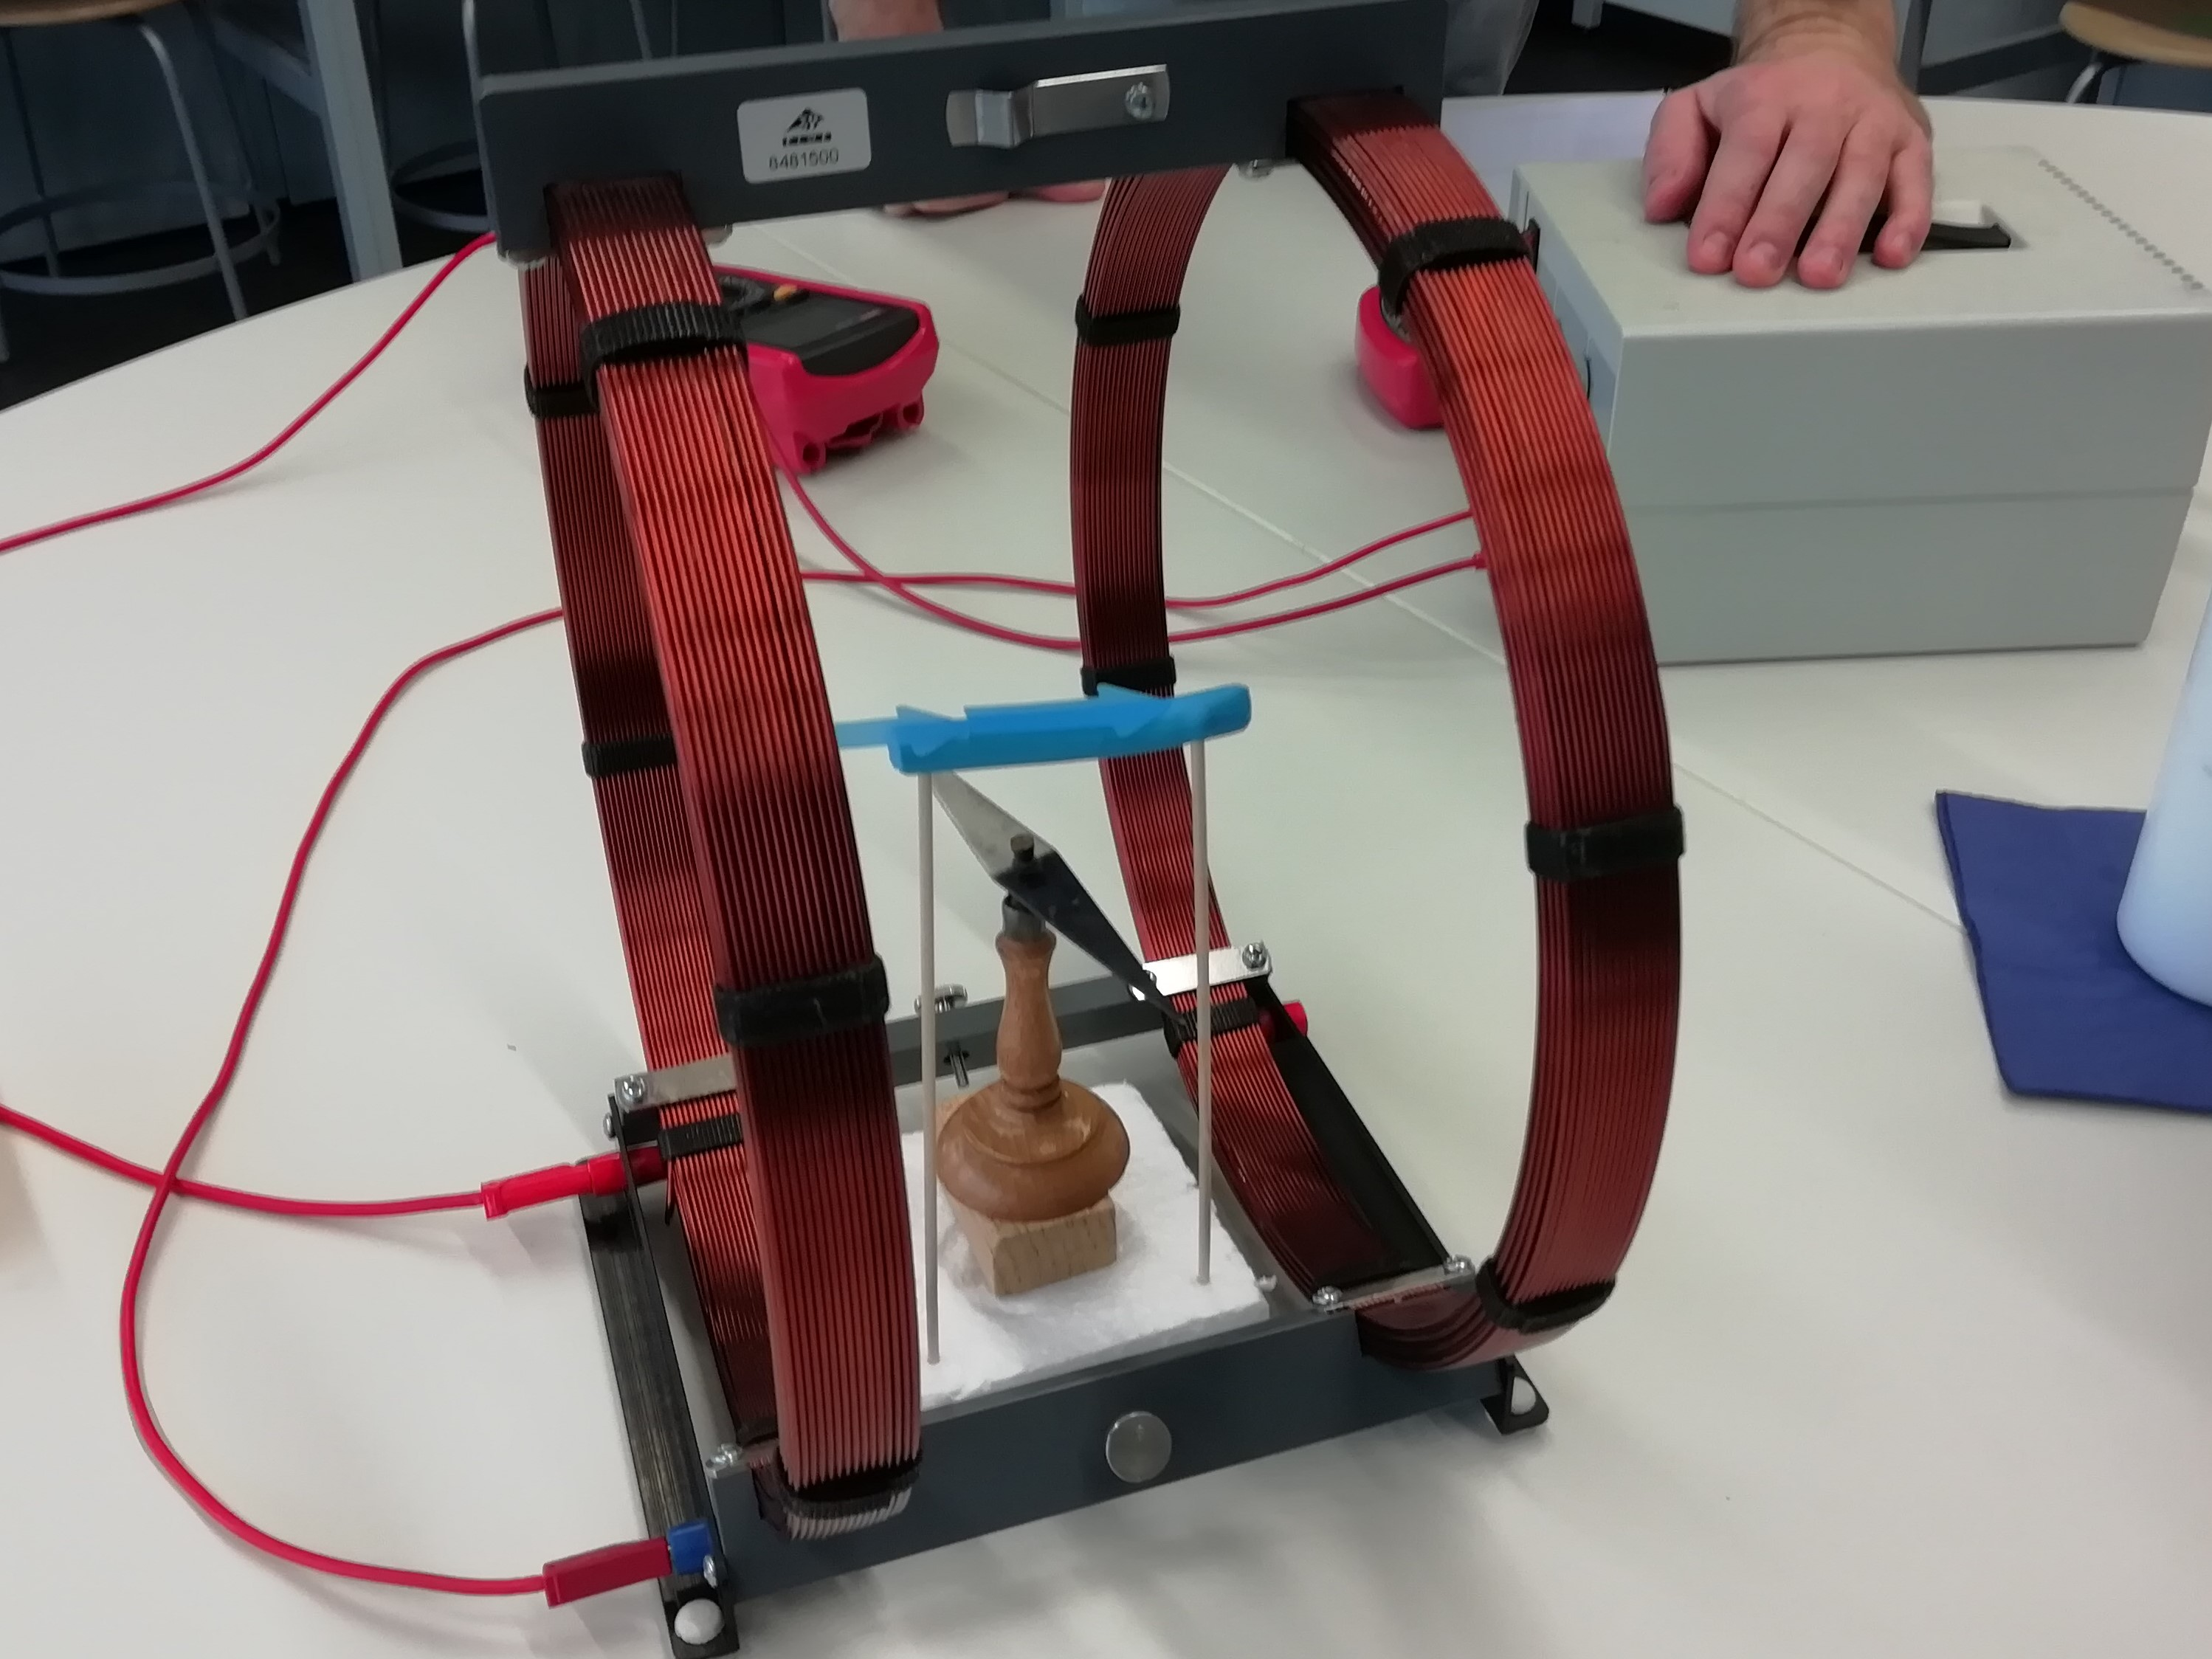
\includegraphics[width=0.4\textwidth]{images/Design_1.jpg}
	\hspace{0.05cm}
	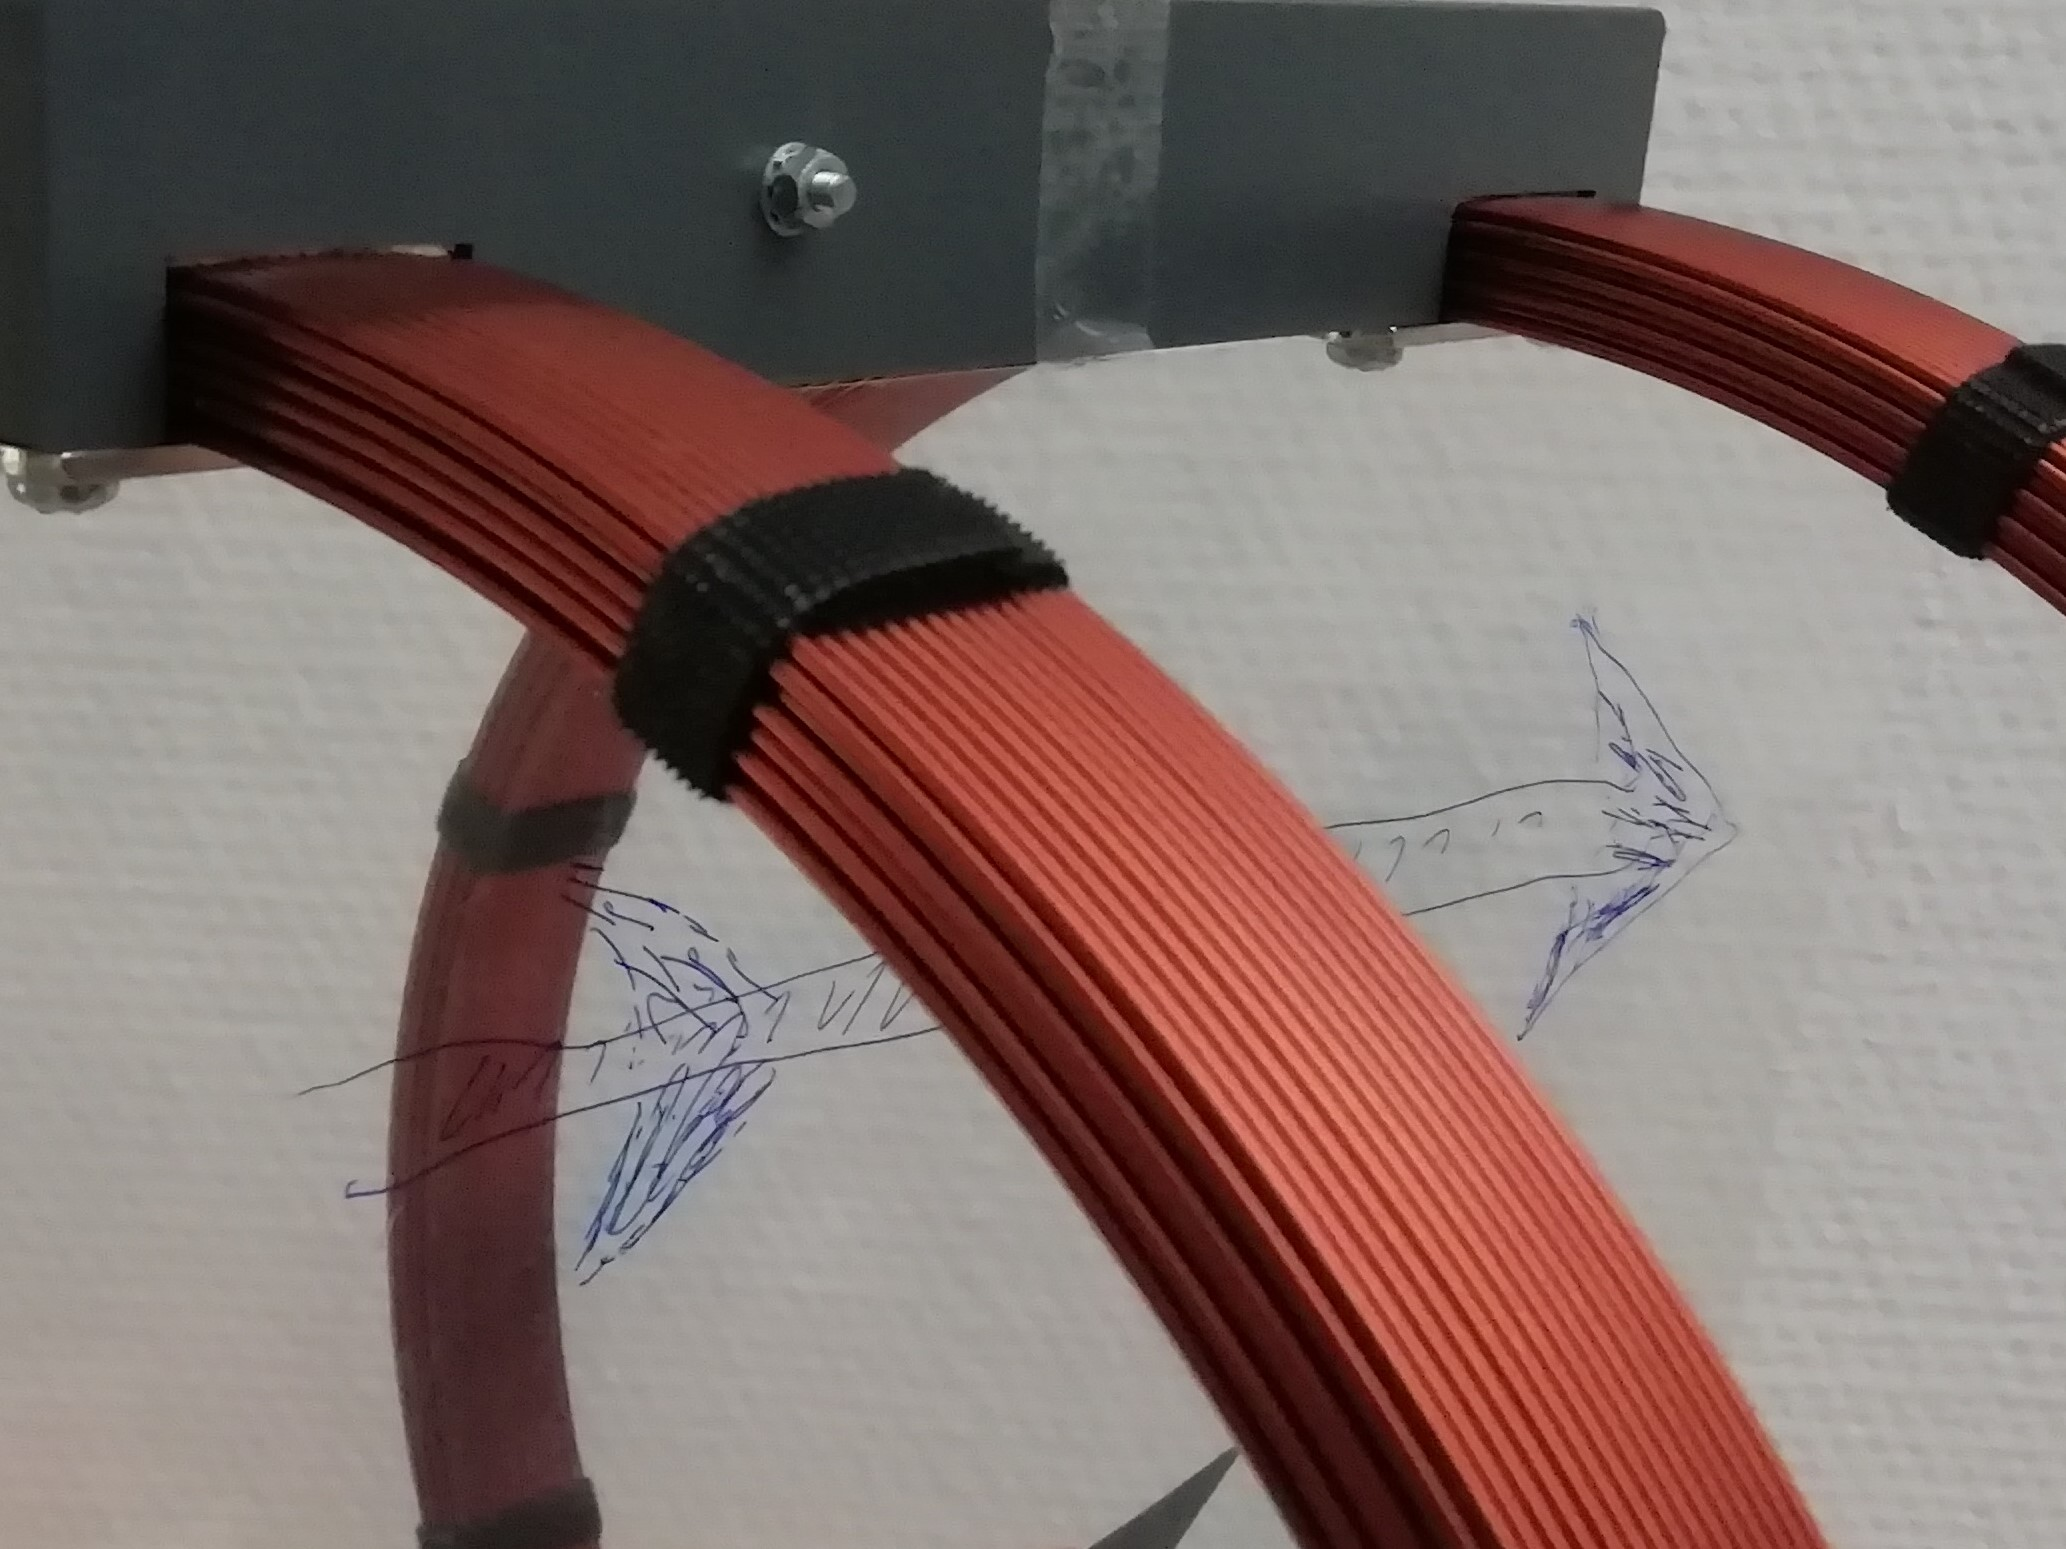
\includegraphics[width=0.4\textwidth]{images/Design_2.jpg}	
	
	
	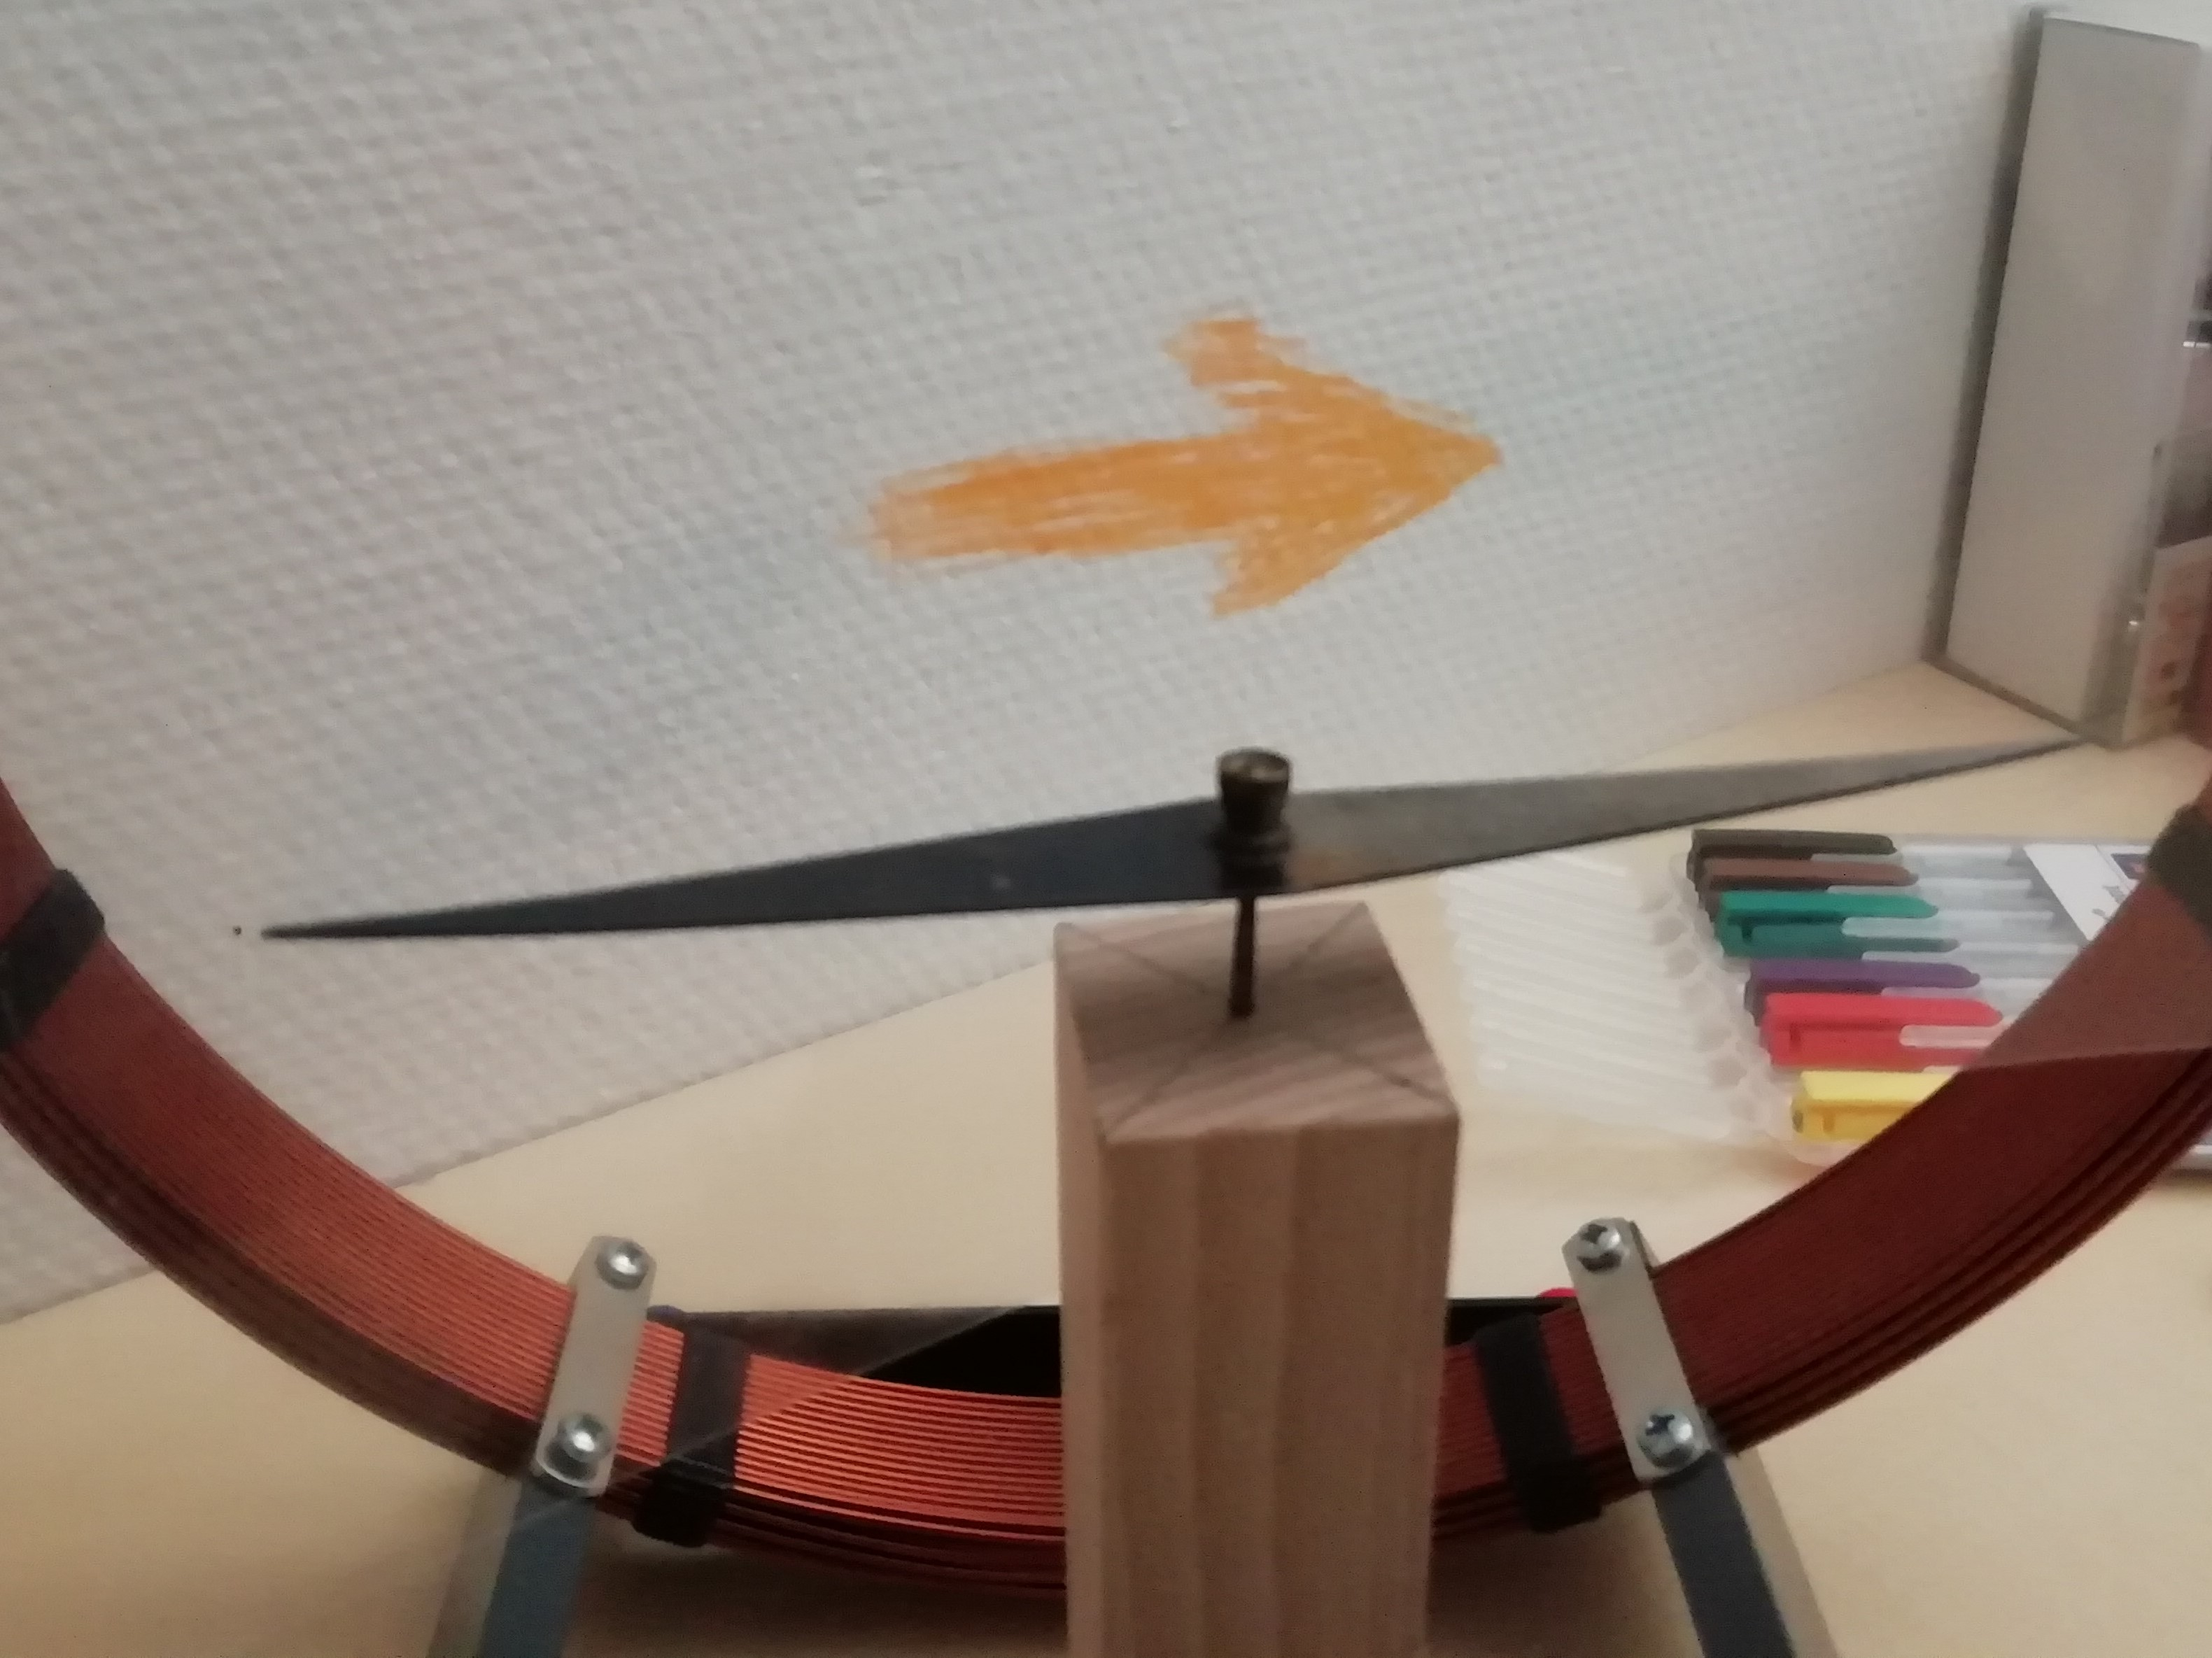
\includegraphics[width=0.4\textwidth]{images/Design_3.jpg}	
	\hspace{0.05cm}
	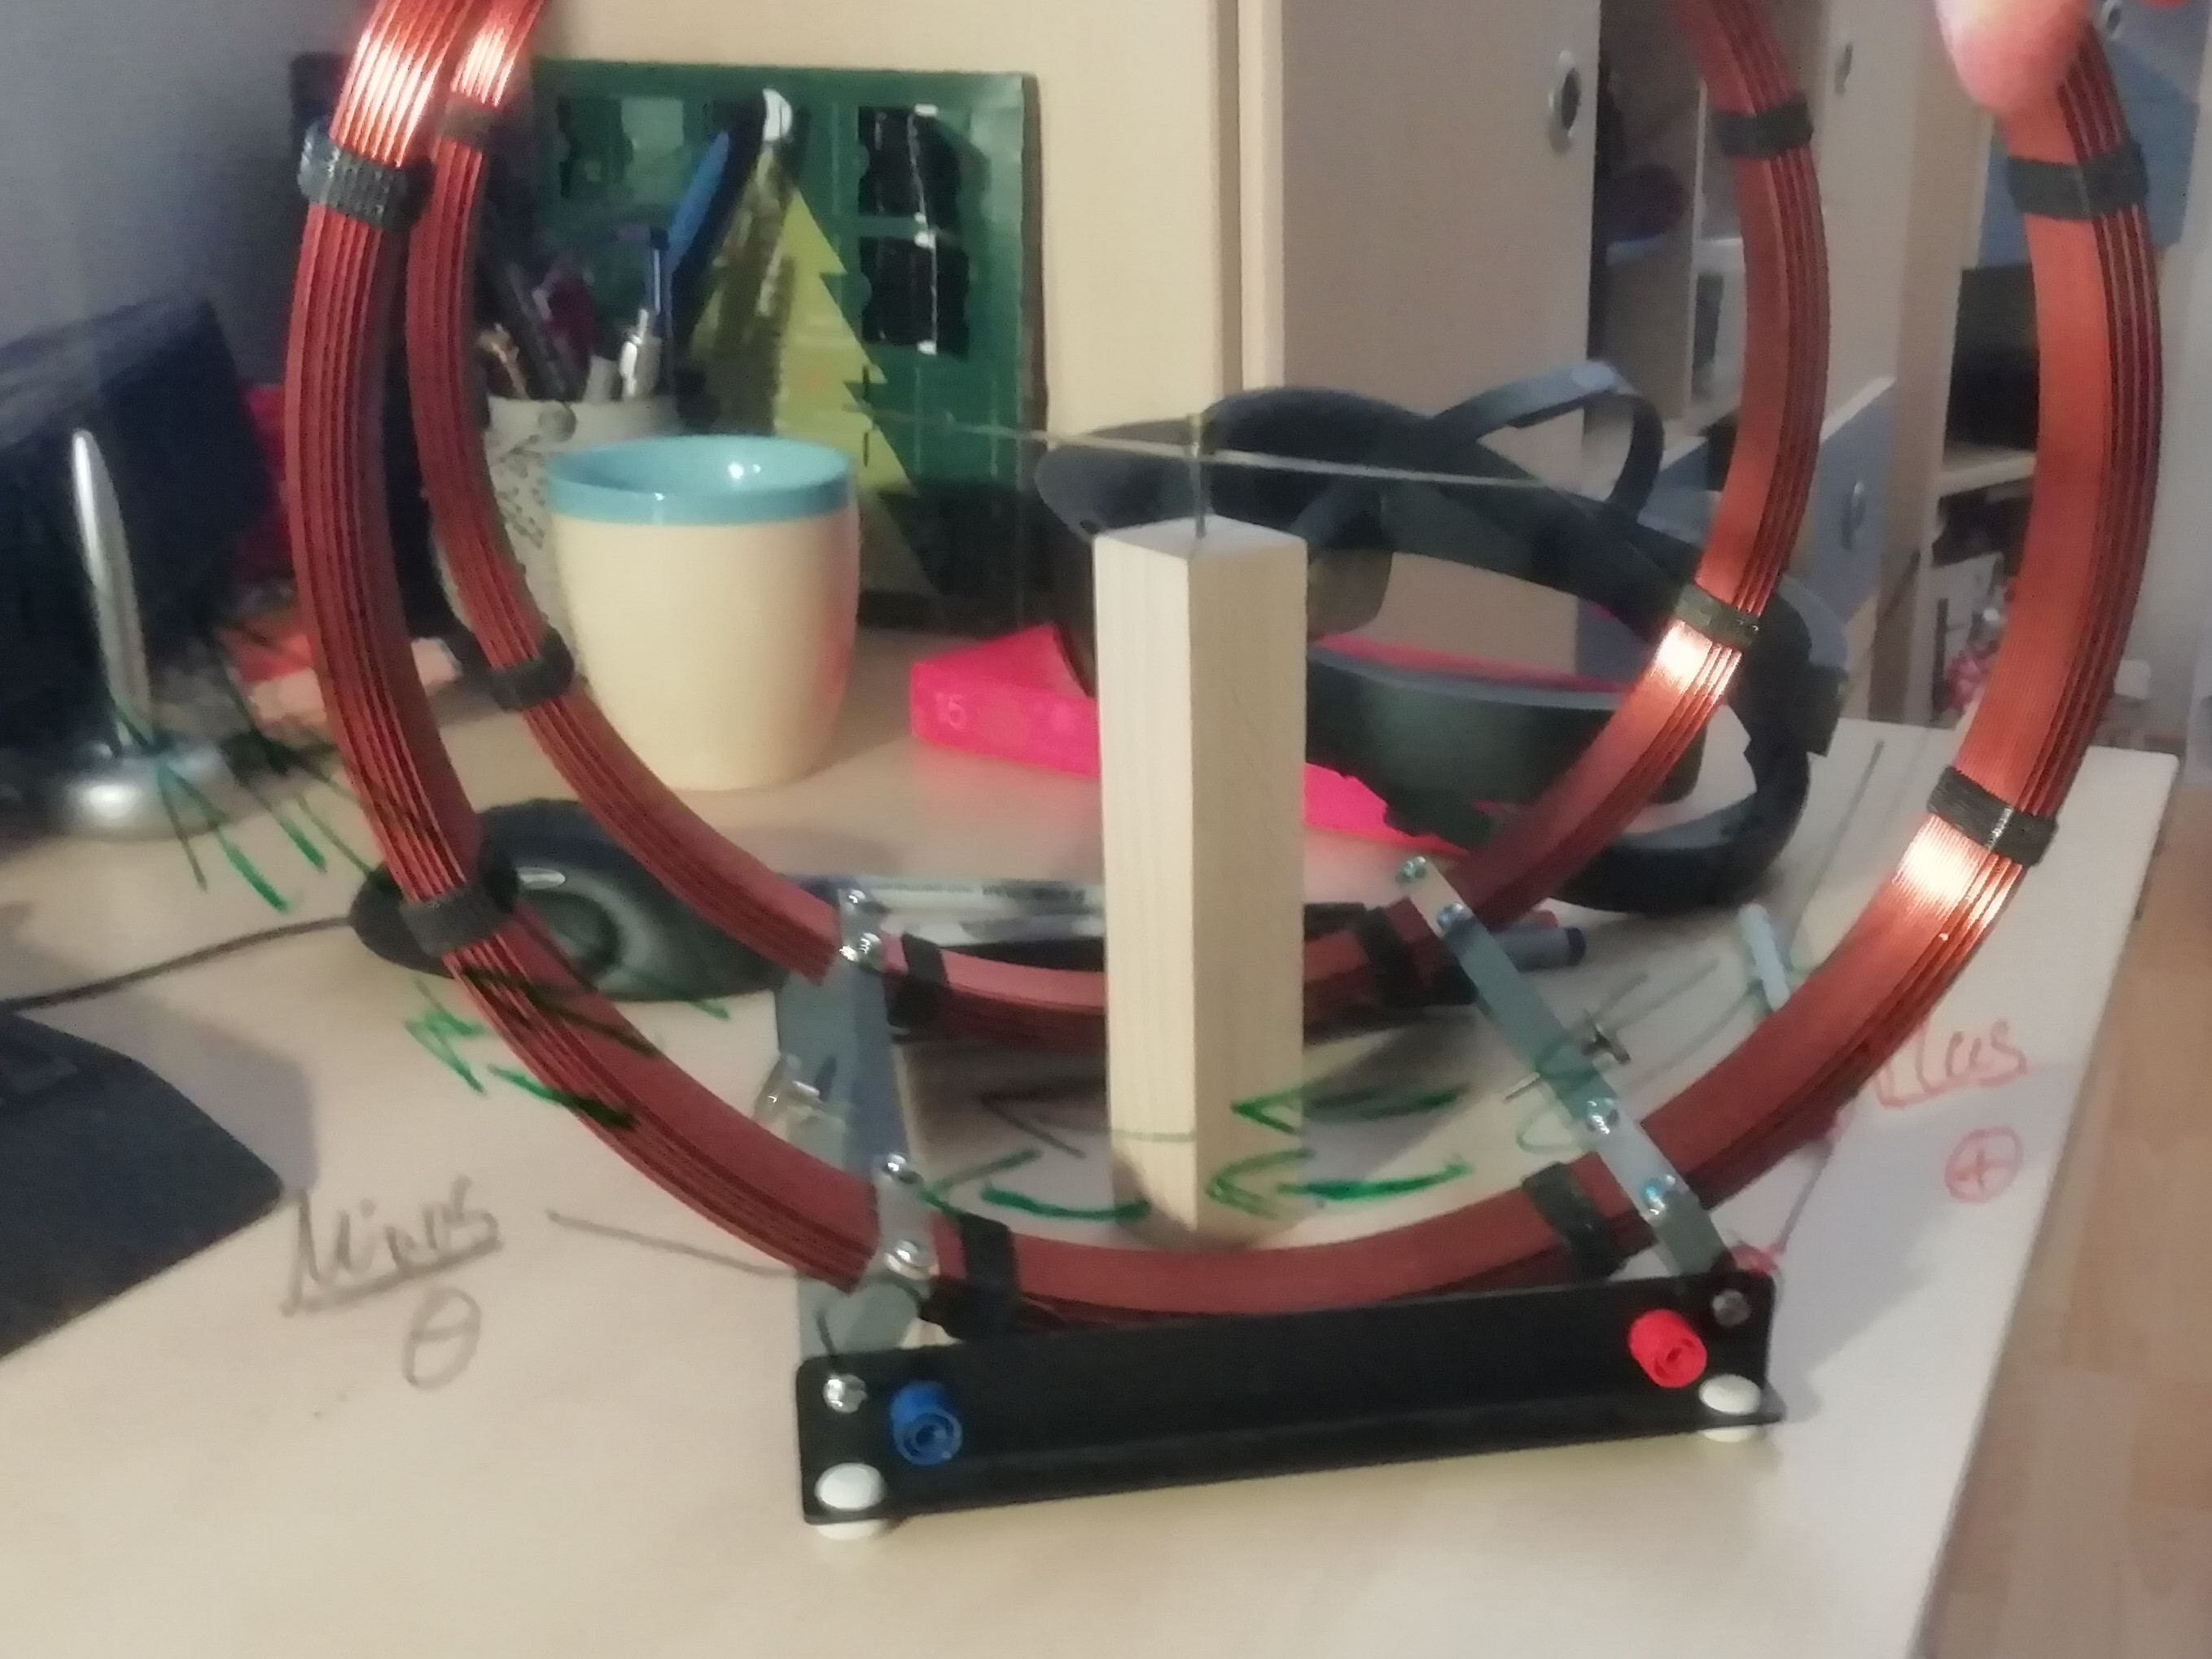
\includegraphics[width=0.4\textwidth]{images/Design_4.jpg}	
\end{center}
\end{frame}

\begin{frame}[fragile]{Ansatz -- Magnetfeld}
\begin{itemize}
\item Magnetfeld als räumlich in die Spule eingebettete, dreidimensionale Geometrie anzeigen
\item Zwei verschiedene schematische Darstellungen für Magnetfeld anbieten: Vektor-Modell und Feldlinien-Modell
\item Einbettung durch Depth Cues unterstützen (in erster Linie Verdeckung der virtuellen Geometrie durch reale Spule)
\item Sensordaten in Echtzeit an HoloLens übermitteln und Geometrie auf dem Device in Echtzeit berechnen und darstellen
\end{itemize}
\end{frame}

\part{Prototyp}
\begin{frame}[fragile]{}
\vspace{-1em}
\begin{center}
	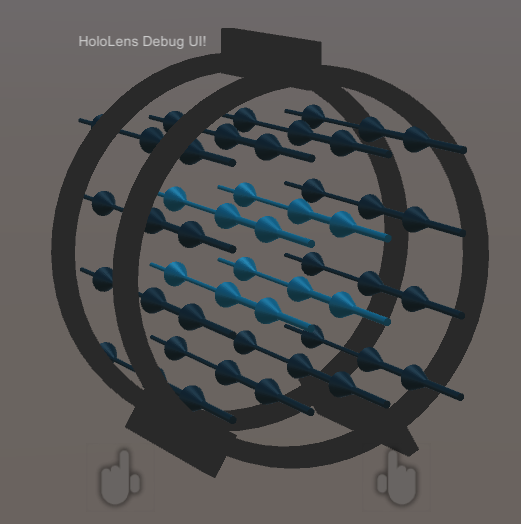
\includegraphics[width=0.3\textwidth]{images/Unity.png}
	\hspace{0.05cm}
	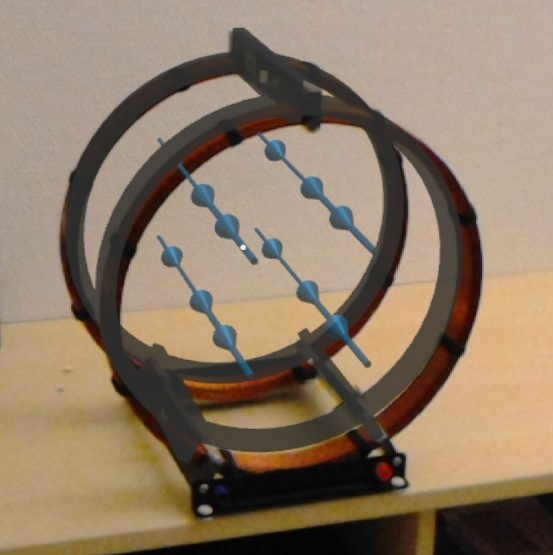
\includegraphics[width=0.3\textwidth]{images/Prototype_Screenshot_1.jpg}
	
	
	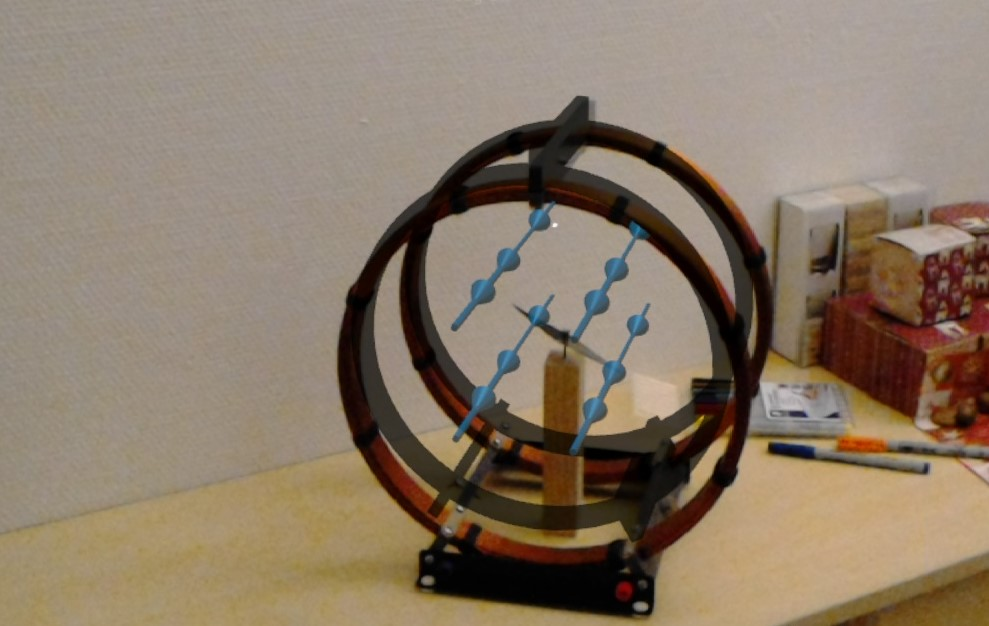
\includegraphics[width=0.4\textwidth]{images/Prototype_Screenshot_2.jpg}	
	\hspace{0.05cm}
	\includegraphics[width=0.4\textwidth]{images/Prototype_Screenshot_5.jpg}
\end{center}
\end{frame}


\part{Umsetzung}
\label{part:practice}
\begin{frame}[fragile]{Technische Umsetzung}
\begin{itemize}
	\item Feldlinien und Vektoren über 3D-Modelle
	\item Verdeckung über ''schwarzes'', virtuelles Modell
	\item Positionierung der virtuellen Objekte über optischen Marker, der einem Tracking-Framework als Anker dient
	\item Sensordaten über Arduino an Laptop, dann über Webserver per WLAN an HoloLens
	\item MSAA für bessere Darstellungen und besseren Text nutzen
\end{itemize}
\end{frame}

\begin{frame}[fragile]{Problemzonen}
\begin{itemize}
	\item Stabilität der Hologramme
	\item Distanz
	\item Performance
	\item Clutter
	\item Details und Fine-Tuning der Visualisierungen
	\item Genauigkeit von Marker-Tracking und Amperemeter-Daten
\end{itemize}
\end{frame}

\begin{frame}[fragile]{Zusammenfassung}
\begin{itemize}
	\item[$\checkmark$] Literaturrecherche
	\item[$\checkmark$] Anforderungen und Probleme herausgearbeitet
	\item[$\checkmark$] Lösungsansatz erarbeitet
	\item[$\checkmark$] Design (grob)
	\item[$\checkmark$] Prototyp mit Basisfunktionaliät
	\item Präzisierung des Designs
	\item Fine-Tuning
	\item Umsetzung weiterer Funktionen
	\item Schriftliche Ausarbeitung
\end{itemize}
\end{frame}

\part{Diskussion}
\begin{frame}[fragile]{}
Vielen Dank für Ihre Aufmerksamkeit!

\vspace{1em}
\hspace{1em} Fragen?
\end{frame}

\part{Quellen}
\begin{frame}[allowframebreaks]
\printbibliography
\end{frame}

\begin{frame}
https://docs.microsoft.com/en-us/windows/mixed-reality/ (Abgerufen am 18.12.2018)

https://de.wikipedia.org/wiki/Helmholtz-Spule (Abgerufen am 18.12.2018)
\end{frame}


